\subsection*{Stop, Question, and Frisk data}

The legal sector is one in which ADMs have been deployed, more often than not accompanied by public debate and protests about targeted policing and racial discrimination (COMPASS as the most popular example). We will turn our focus to the stop, question, and frisk (SQF) dataset published by the New York police department (NYPD). A. Fabris and S. Messina and G. Silvello and G.A. Susto scanned more than x datasets to diversify the datasets that are used in the fairness literature. They recommend it as suitable dataset for fairness research. First, we will give some context to the dataset. We will continue with descriptive analysis and finally examine fairness of an algorithm trained on this data.

Since x the stop, question, and frisk practice is implemented in New York City. A police officer is allowed to stop a person if they have reasonable suspicion that the person has committed, is committing, or is about to commit a crime.
During the stop the officer is allowed to frisk a person (pat-down the person's outer clothing) or search them more carefully.
The stop can result in a summon, an arrest or no further consequences. After a stop was made, the officer is required to fill out a form, documenting the stop. This data is published yearly by the NYPD.
Many citizens have criticized the stop and frisk practice. There is disagreement about whether the strategy is effective in reducing the crime rates of the city {\color{red}cite some studies}. The police has been repeatedly criticized for over-targetting people of colour.
Stop and Frisk practice during 2004 to 2012 has been deemed as unconstitutional. {\color{red} Source}

\subsubsection*{Data description}
For our analysis we look at the stops from 2023 as they were the most recent at the time of writing this paper. The raw 2023 dataset consists of 16971 observations and 82 variables. We first discarded all the variables that have more than 20\% missing values, which leaves 34 variables.
From this reduced dataset we filter out the complete cases and end up with 12039 observations. \footnote{Simply discarding the missing values and only training on complete cases is discouraged by \cite{fernando2021}. We opt for this approach regardless, since imputation of the missing values is not straight forward
but treating missing values as an extra category (which some random forest learners in mlr3 can do) will introduce complications when we implement some fairness methods later on.}

% (many fairness methods can not deal with missing data, especially in the protected attribute, which makes sense, since they base their decision on it). 
Race is the protected attribute (PA). For the fairness audit later in the chapter we dichotomize the PA to adjust our situation to the common binary classification, binary PA scenario in the fairness literature. For a more nuanced descriptive analysis we only summarize "Black Hispanic" and "Black" into the group "Black" and  "American Indian/ Native American" and "Middle Eastern/ Southwest Asian" into the "Other" category.  
Black people are by far most often stopped, making up 70\% of the total stops; yet, according to 2020 census data black people make up only 20\% of the city's population \autoref{fig:race_distributions}. At the same time white people form the majority of New York citizens (30\%) but contribute with only 6\% to the stops. 
After 2021 there has been a stark decline in stops and the police is known to focus their attention on high crime areas. Therefore, we further look at each borough. 
The most stops in 2023 occur in Bronx and Brooklyn. Based on report of the NYPD and population statistics from 2020, the Bronx also has the highest estimated crime rate per 100,000 citizens. Manhattan is not far behind in crime rate, but has fewer stops. Note that Bronx and Brooklyn happen to be the boroughs with the highest proportion of black citizens \autoref{fig:nyc_pop_crimerates_stops_comparison}. 
\begin{figure}
  \centering
  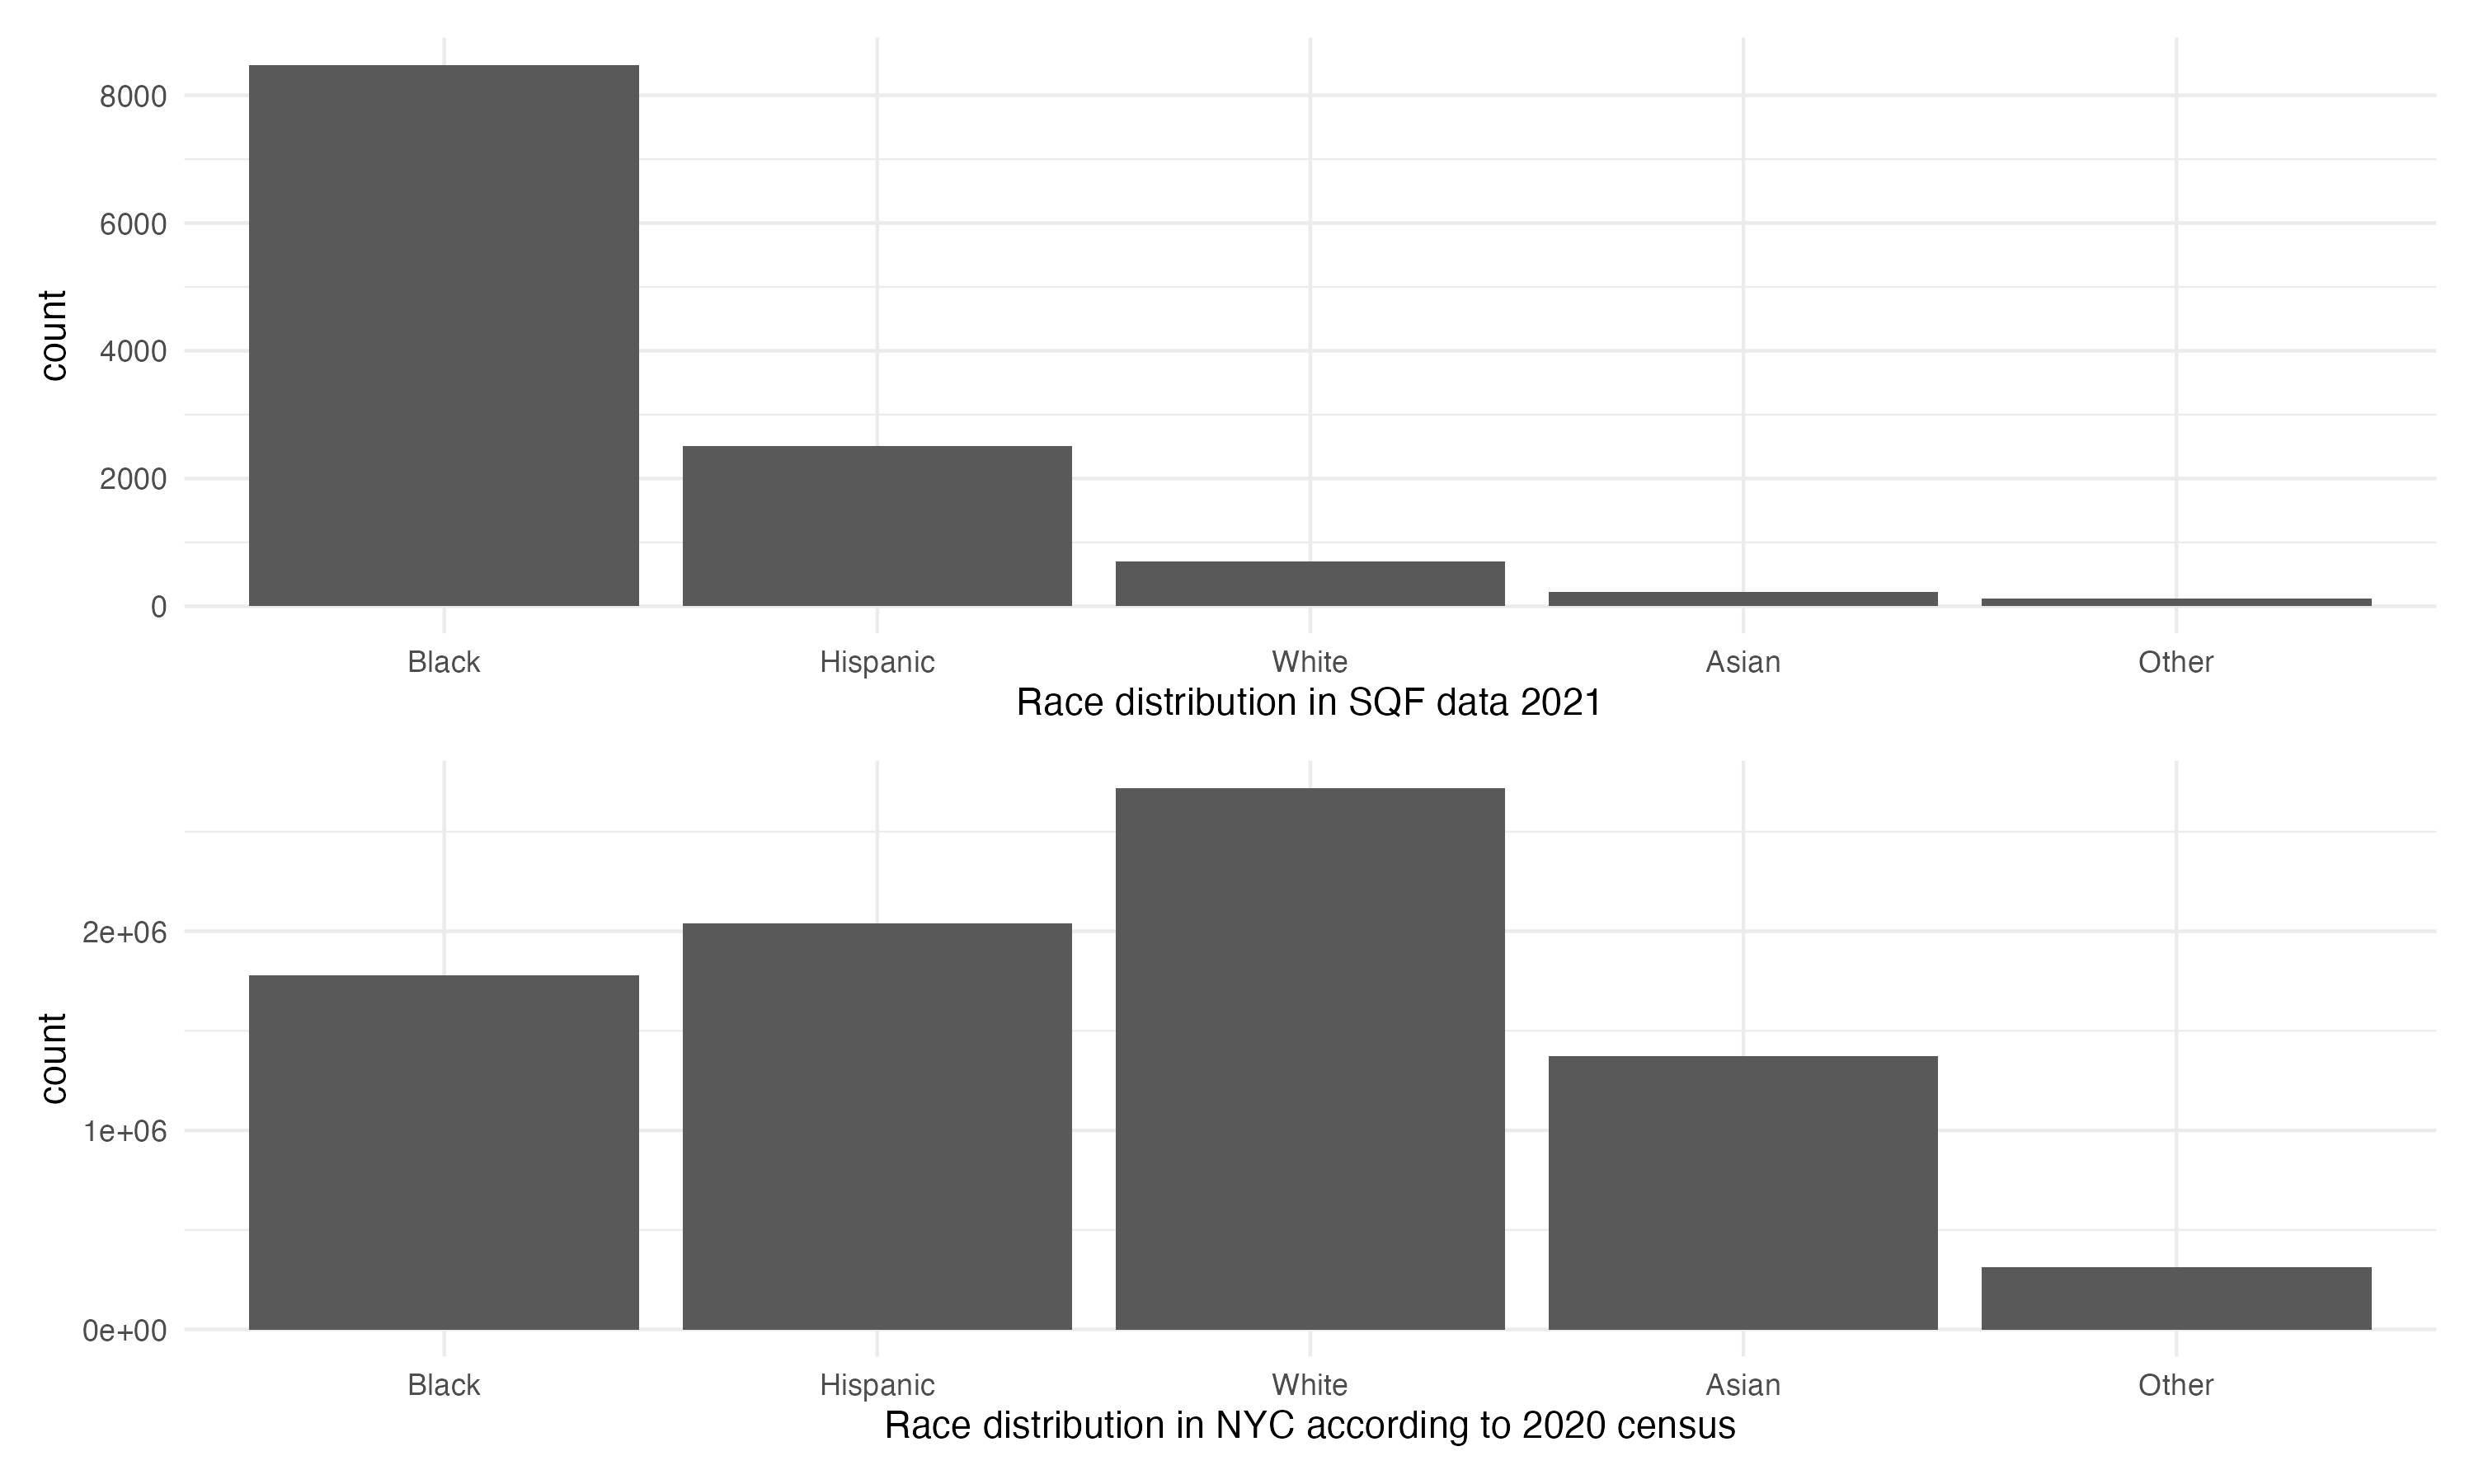
\includegraphics[width=0.7\textwidth]{../figures/sqf_case_study_plot6.png}
  \caption{Comparison of race distribution in the training and target population.}
  \label{fig:race_distributions}
\end{figure}

\begin{figure}
    \centering
    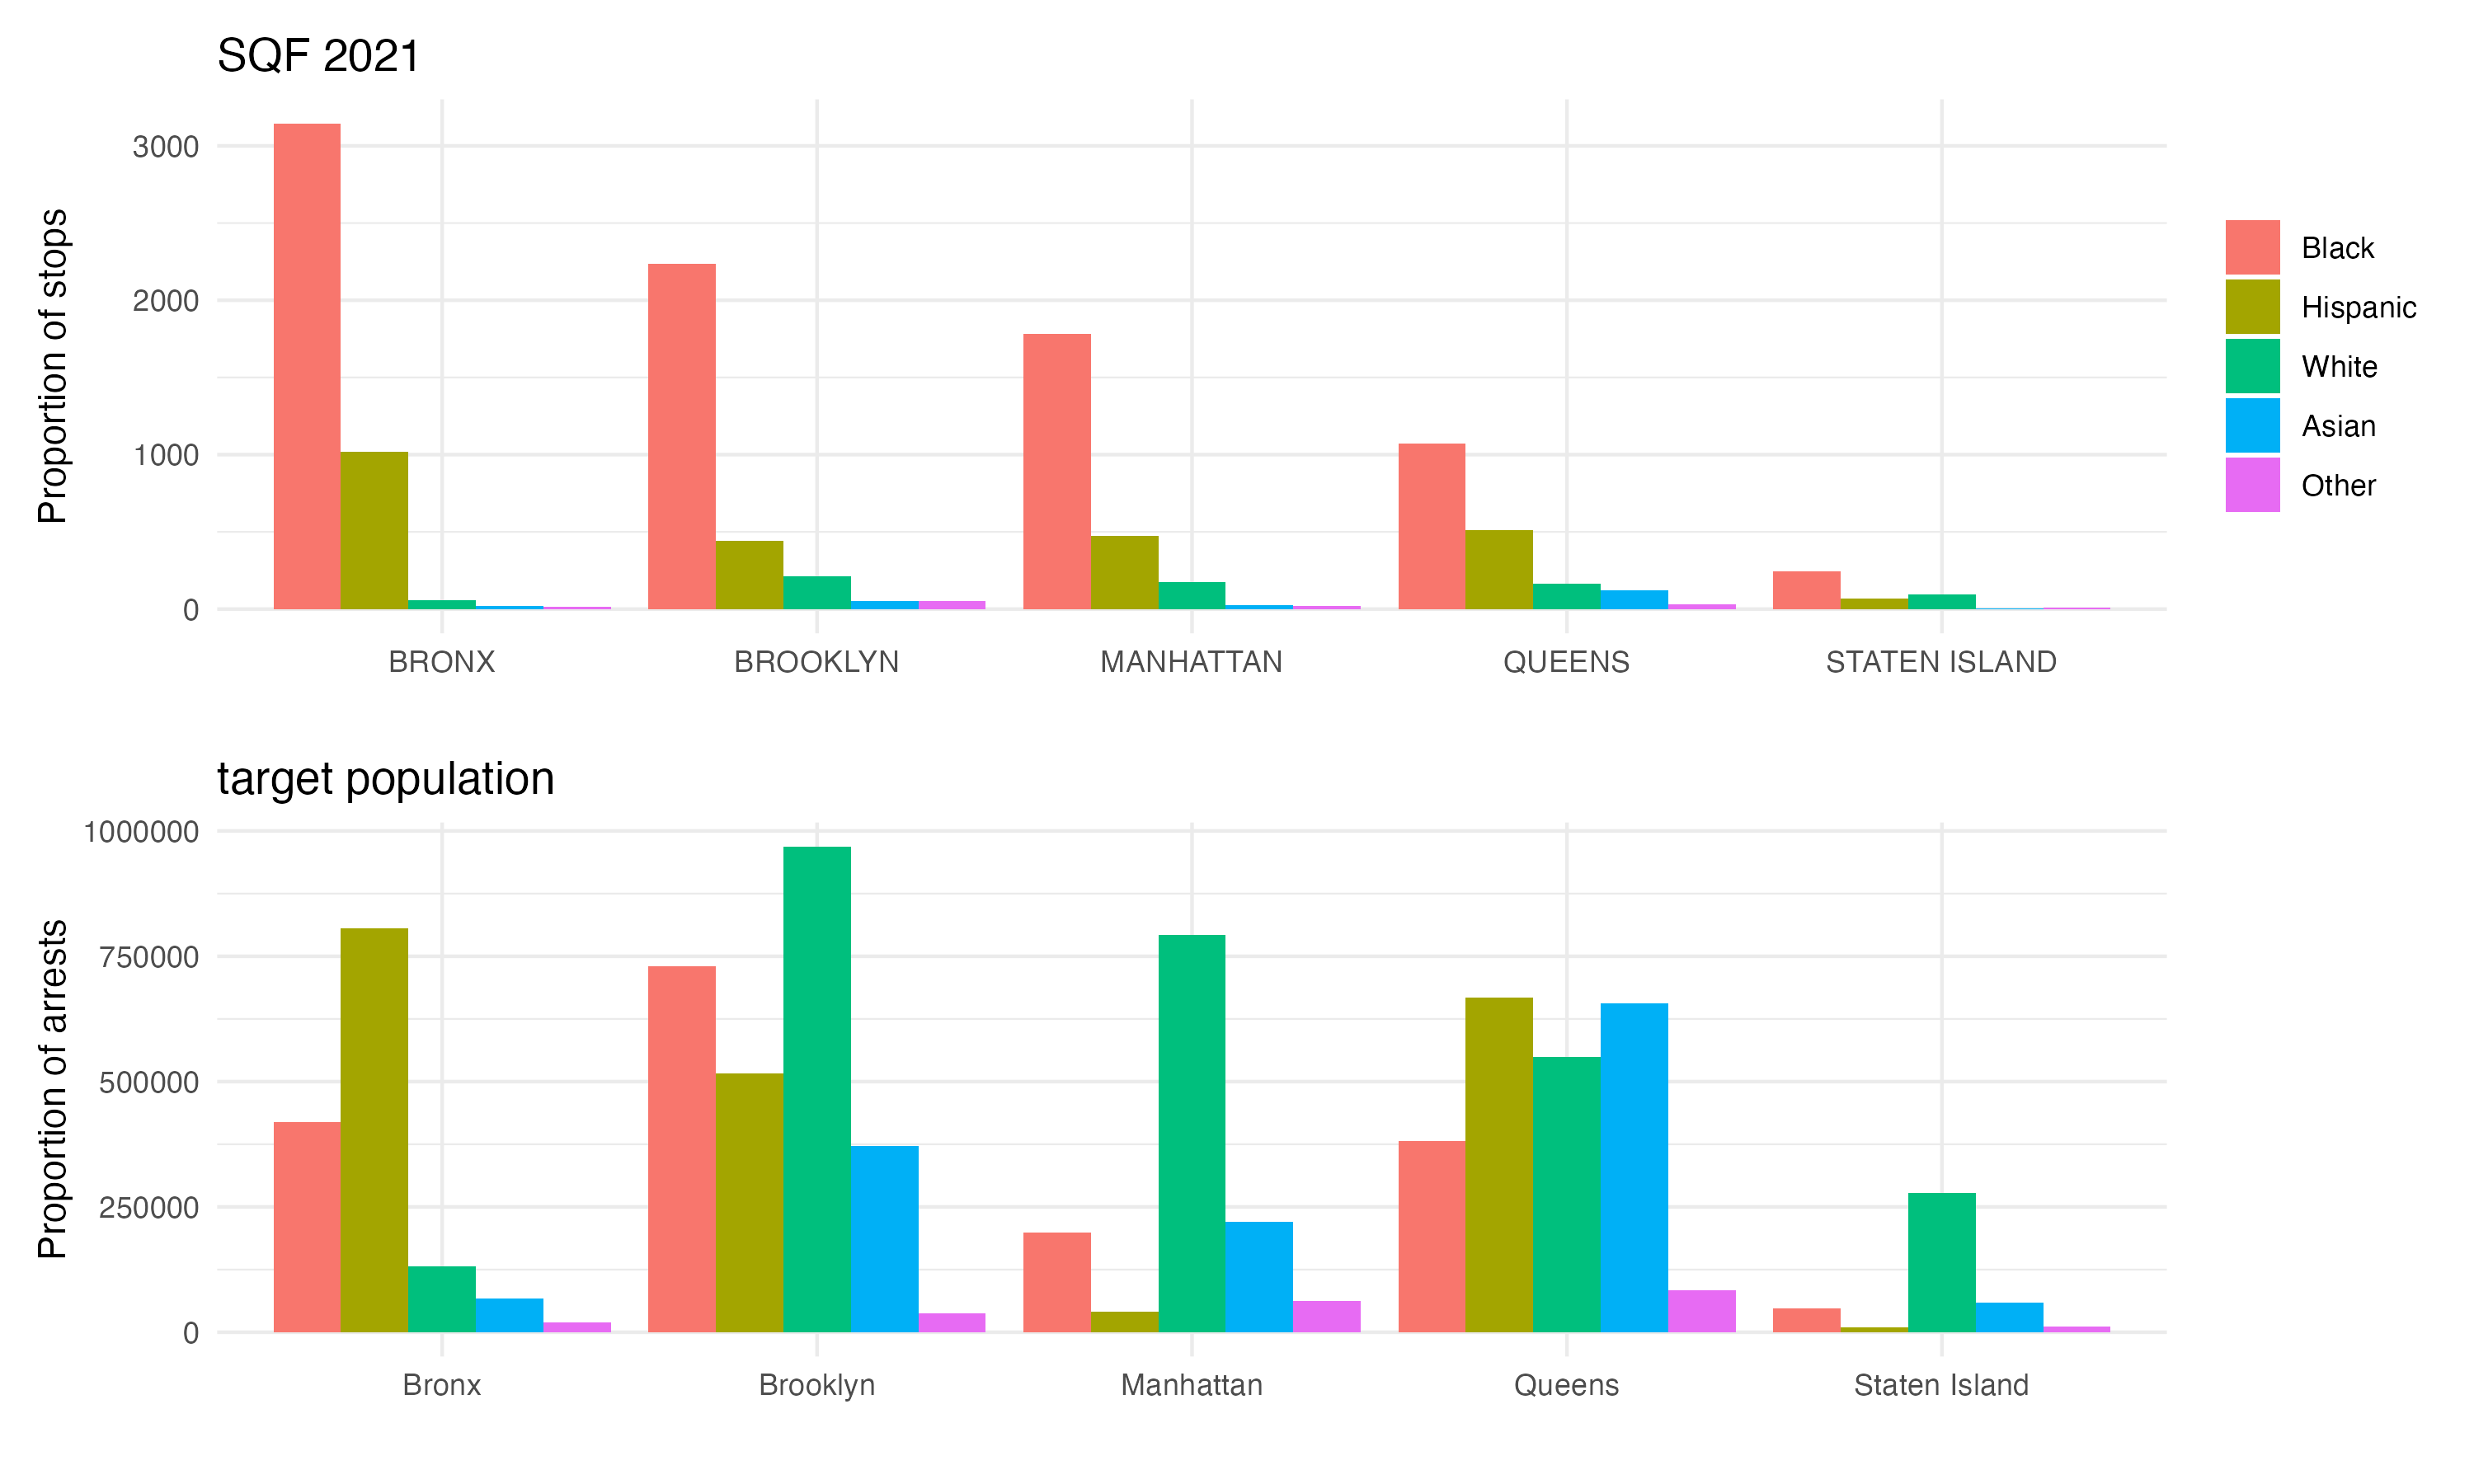
\includegraphics[width=0.7\textwidth]{../figures/sqf_case_study_plot11.png}
    \caption{Racial distribution in the SQF data of each borough in comparison to the racial distribution of each borough in NYC as a whole.}
    \label{fig:racial_distribution_borough}
\end{figure}
\begin{figure}
    \centering
    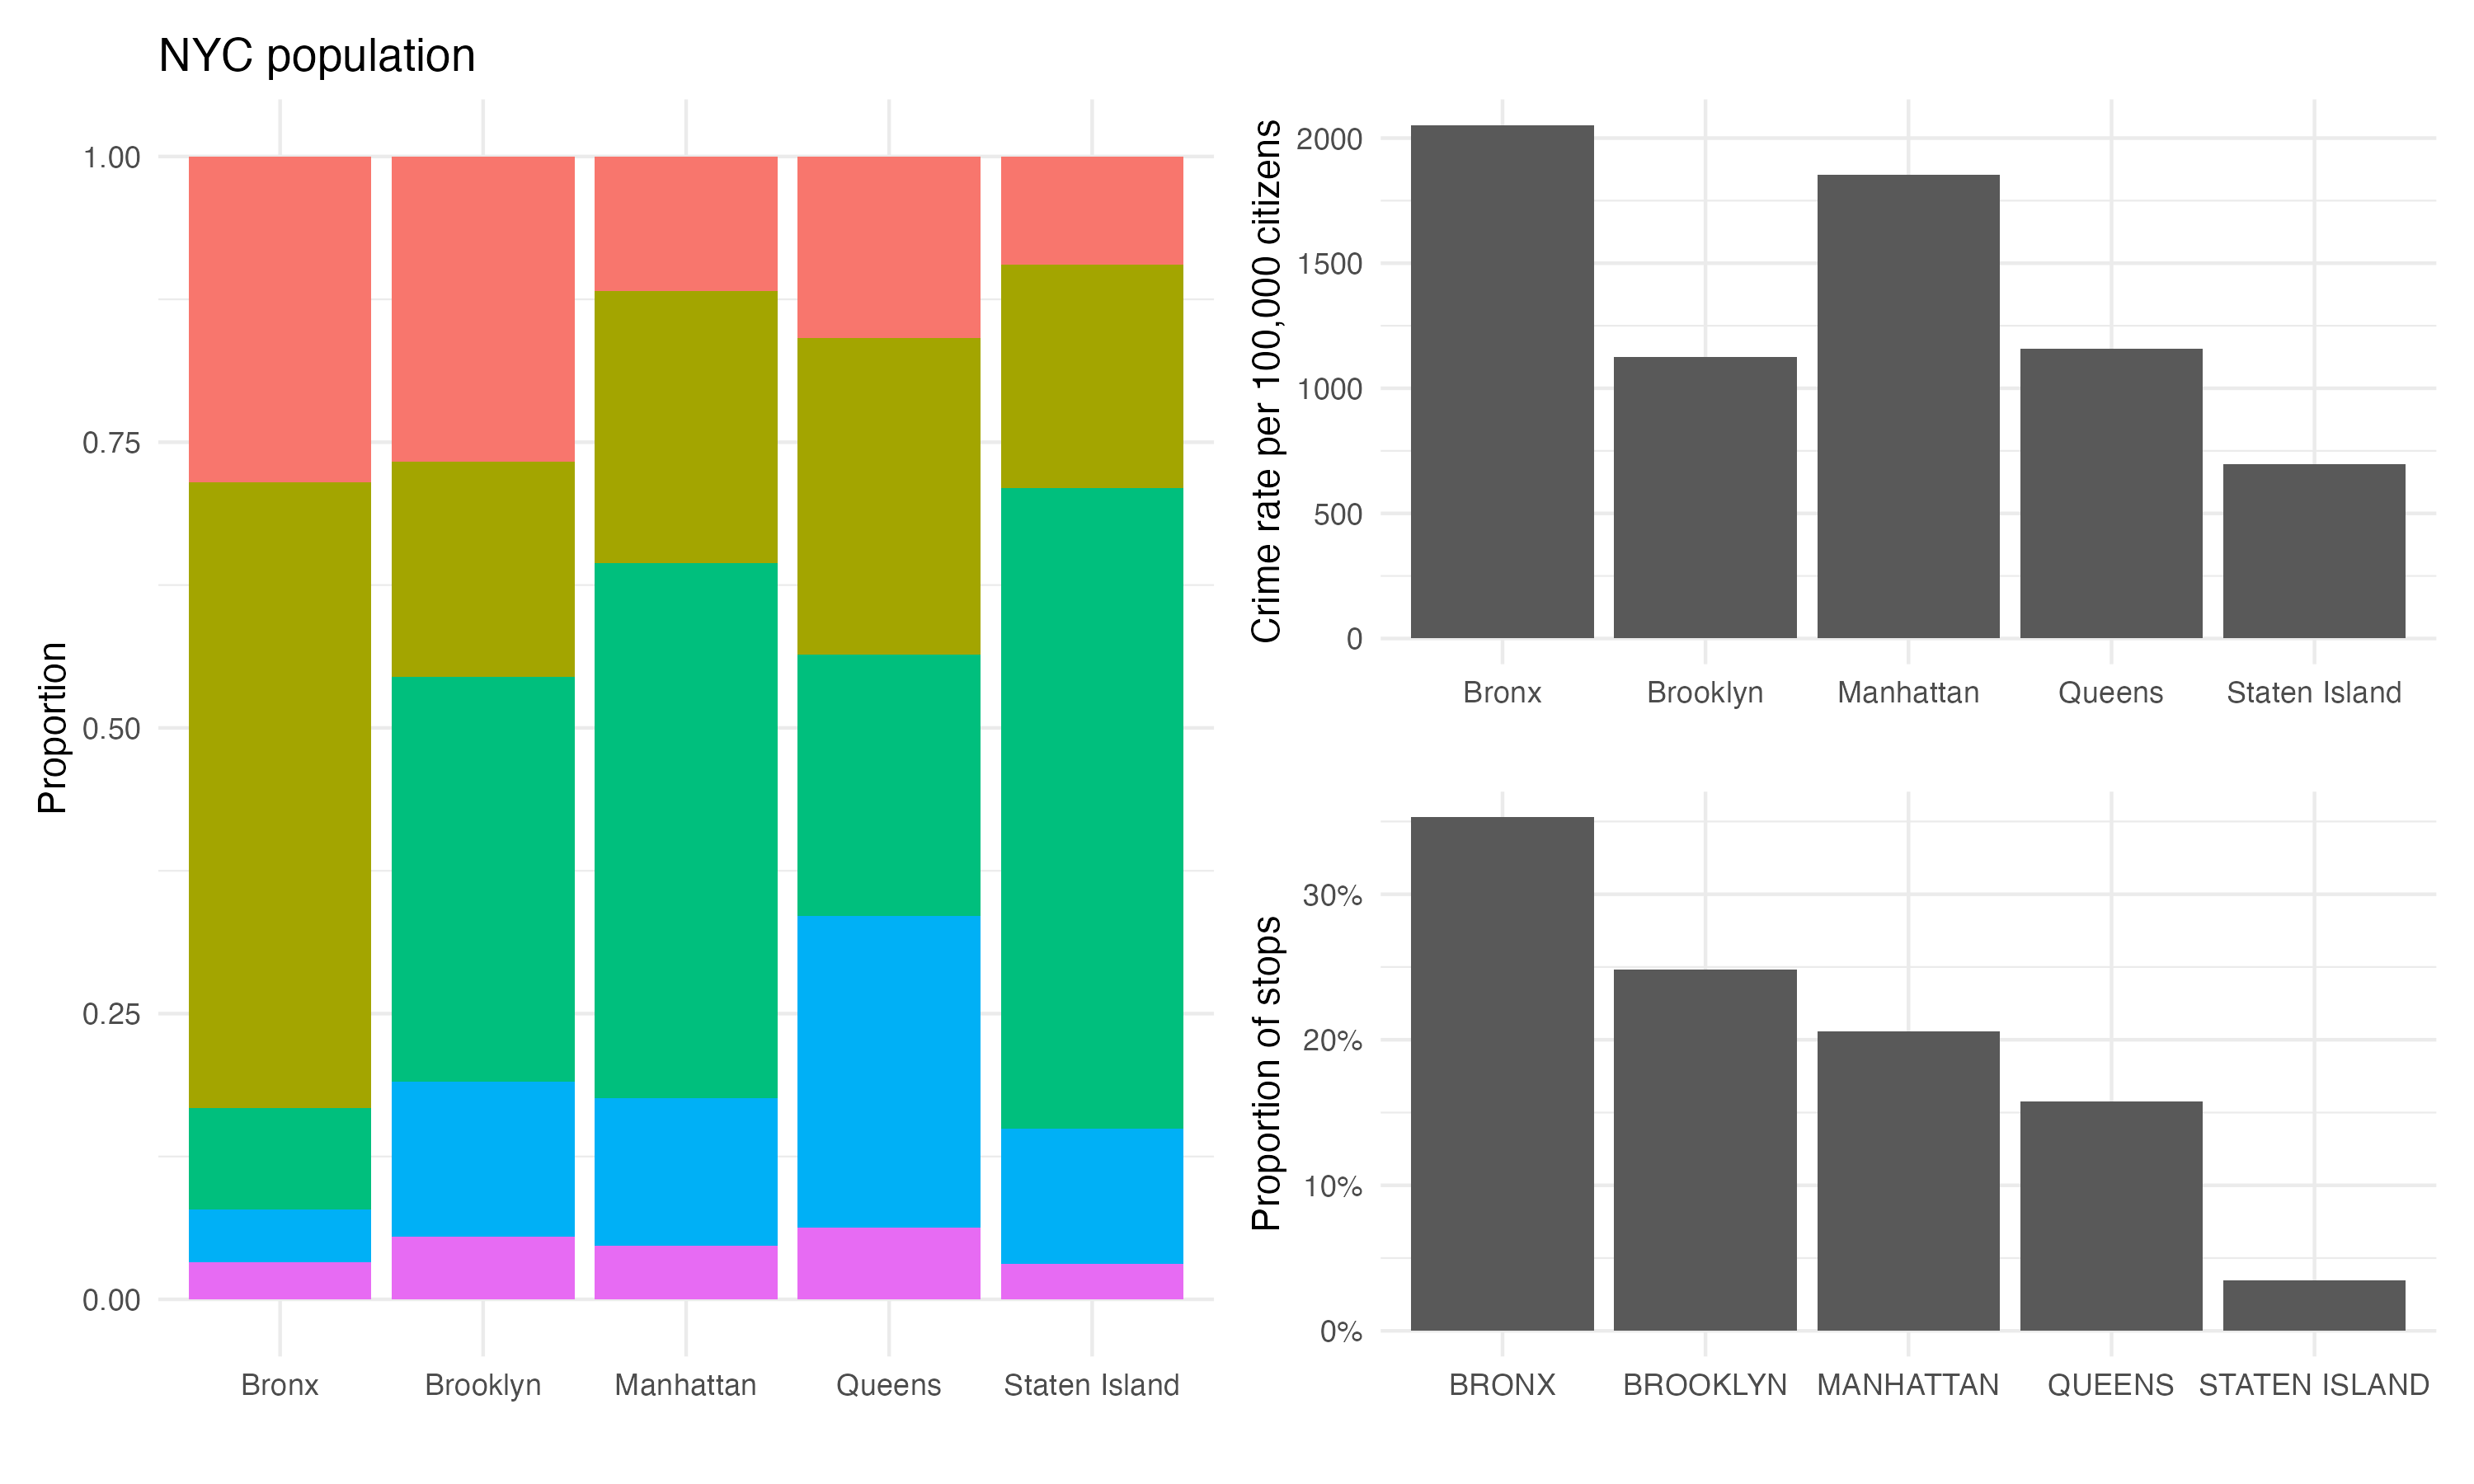
\includegraphics[width=0.7\textwidth]{../figures/sqf_case_study_plot14.png}
    \caption{Racial distribution in the SQF data of each borough in comparison to the racial distribution of each borough in NYC as a whole.}
    \label{fig:nyc_pop_crimerates_stops_comparison}
\end{figure}

After a more general overview of the dataset, we turn to the outcome of the stop. Specifically, we are interested in the arrestment of a suspect. In the cleaned 2023 data about 31\% of stops result in an arrest.
Overall racial disparities in arrestment rates are low. The arrestment rate for white suspects is the highest. \autoref{fig:arrestment_rates_clean_data}. As group fairness metrics are observational and constructed from the joint probability of $Y, \hat{Y}, A$, this already gives us a hint that the classifier trained to predict the arrestment of a suspect might show little racial disparities.

\subsubsection*{Fairness Auditing}
To train a random forest classifier on the 2023 data to predict the arrest of a person, we dichotomize the race attribute by grouping "Black" and "Hispanic" as people of colour ("PoC") and "White", "Asian", and "Other" as white ("White").
As features, we select variables that should resemble the information that were available to the officer at the time of the stop. Additionally, we control for factors, such as the time of the stop or whether the officer was wearing a uniform. This selection of features is inspired by previous studies on SQF data (e.g. \cite{goel2016}). With many of the group fairness metrics implemented in \texttt{mlr3fairness}, we can measure the (group) fairness of the regular random forest classifier.\\
First we plot the prediction score densities for each group in \autoref{fig:fairness_density}. We can see that in general white people tend to have higher predicted probabilities than PoC. There is a relatively large proportion of PoC with low predicted probabilities, as seen by the peak at around 0.05. Recall that the predicted probability resembles the probability of being predicted positive (arrested).
In \autoref{fig:fairness_metrics} we plot the absolute difference in common group fairness metrics.
Exact equality of the group metrics cannot be expected in practice, so it is common to allow for a margin of error $\epsilon$. Taking $\epsilon = 0.05$, the classifier is fair according to equalized odds, predictive parity, and equal opportunity. The classifier is unfair according to overall accuracy equality and predictive equality. This again shows that there is not one clear solution to fairness, but it depends on the perspective one takes.\\
With the absolute differences alone, it is possible to quantify the magnitude of unfairness but not the direction of it. Thus, we report the group-wise error metrics in \autoref{tab:groupwise_metrics_2023}.
% Interpretation of the direction is, however, not super clear. The positive prediction (to get arrested) is undesirable for the individual, but when a group as a whole has a high proportion of positive predictions, it speaks for the fact that the members were stopped for a good reason. This argumentation follows the principle of assessing a policing strategy based on hit rates. A hit is an arrest and high a high hit rate means that the police is stopping the right people.
% With this ambiguity in mind, we take a closer look at
% We therefore mainly notice the differences in fairness metrics and do not make clear statements about who is discriminated against.
White people have a higher true positive rate, but also a higher false positive rate. This is usually a natural trade-off in classification tasks. For PoC the negative predictive values and the positive predictive value is higher. This means that given a person of colour is predicted as arrested, it is more likely that they were indeed arrested. The same for a negative prediction. Additionally, the false discovery rate, the proportion of predicted positives that are actually negative, is lower for PoC. This means that the classifier is more conservative in predicting positive outcomes for PoC. Overall, the accuracy is higher for PoC.
Apart from the lower true positive rate, one could say that the classifier performs better for PoC than for white people. We will leave this interpretation as it is for now and will return to an alternative view later on.


\begin{figure}
    \centering
    \begin{minipage}{0.48\textwidth}
        \centering
        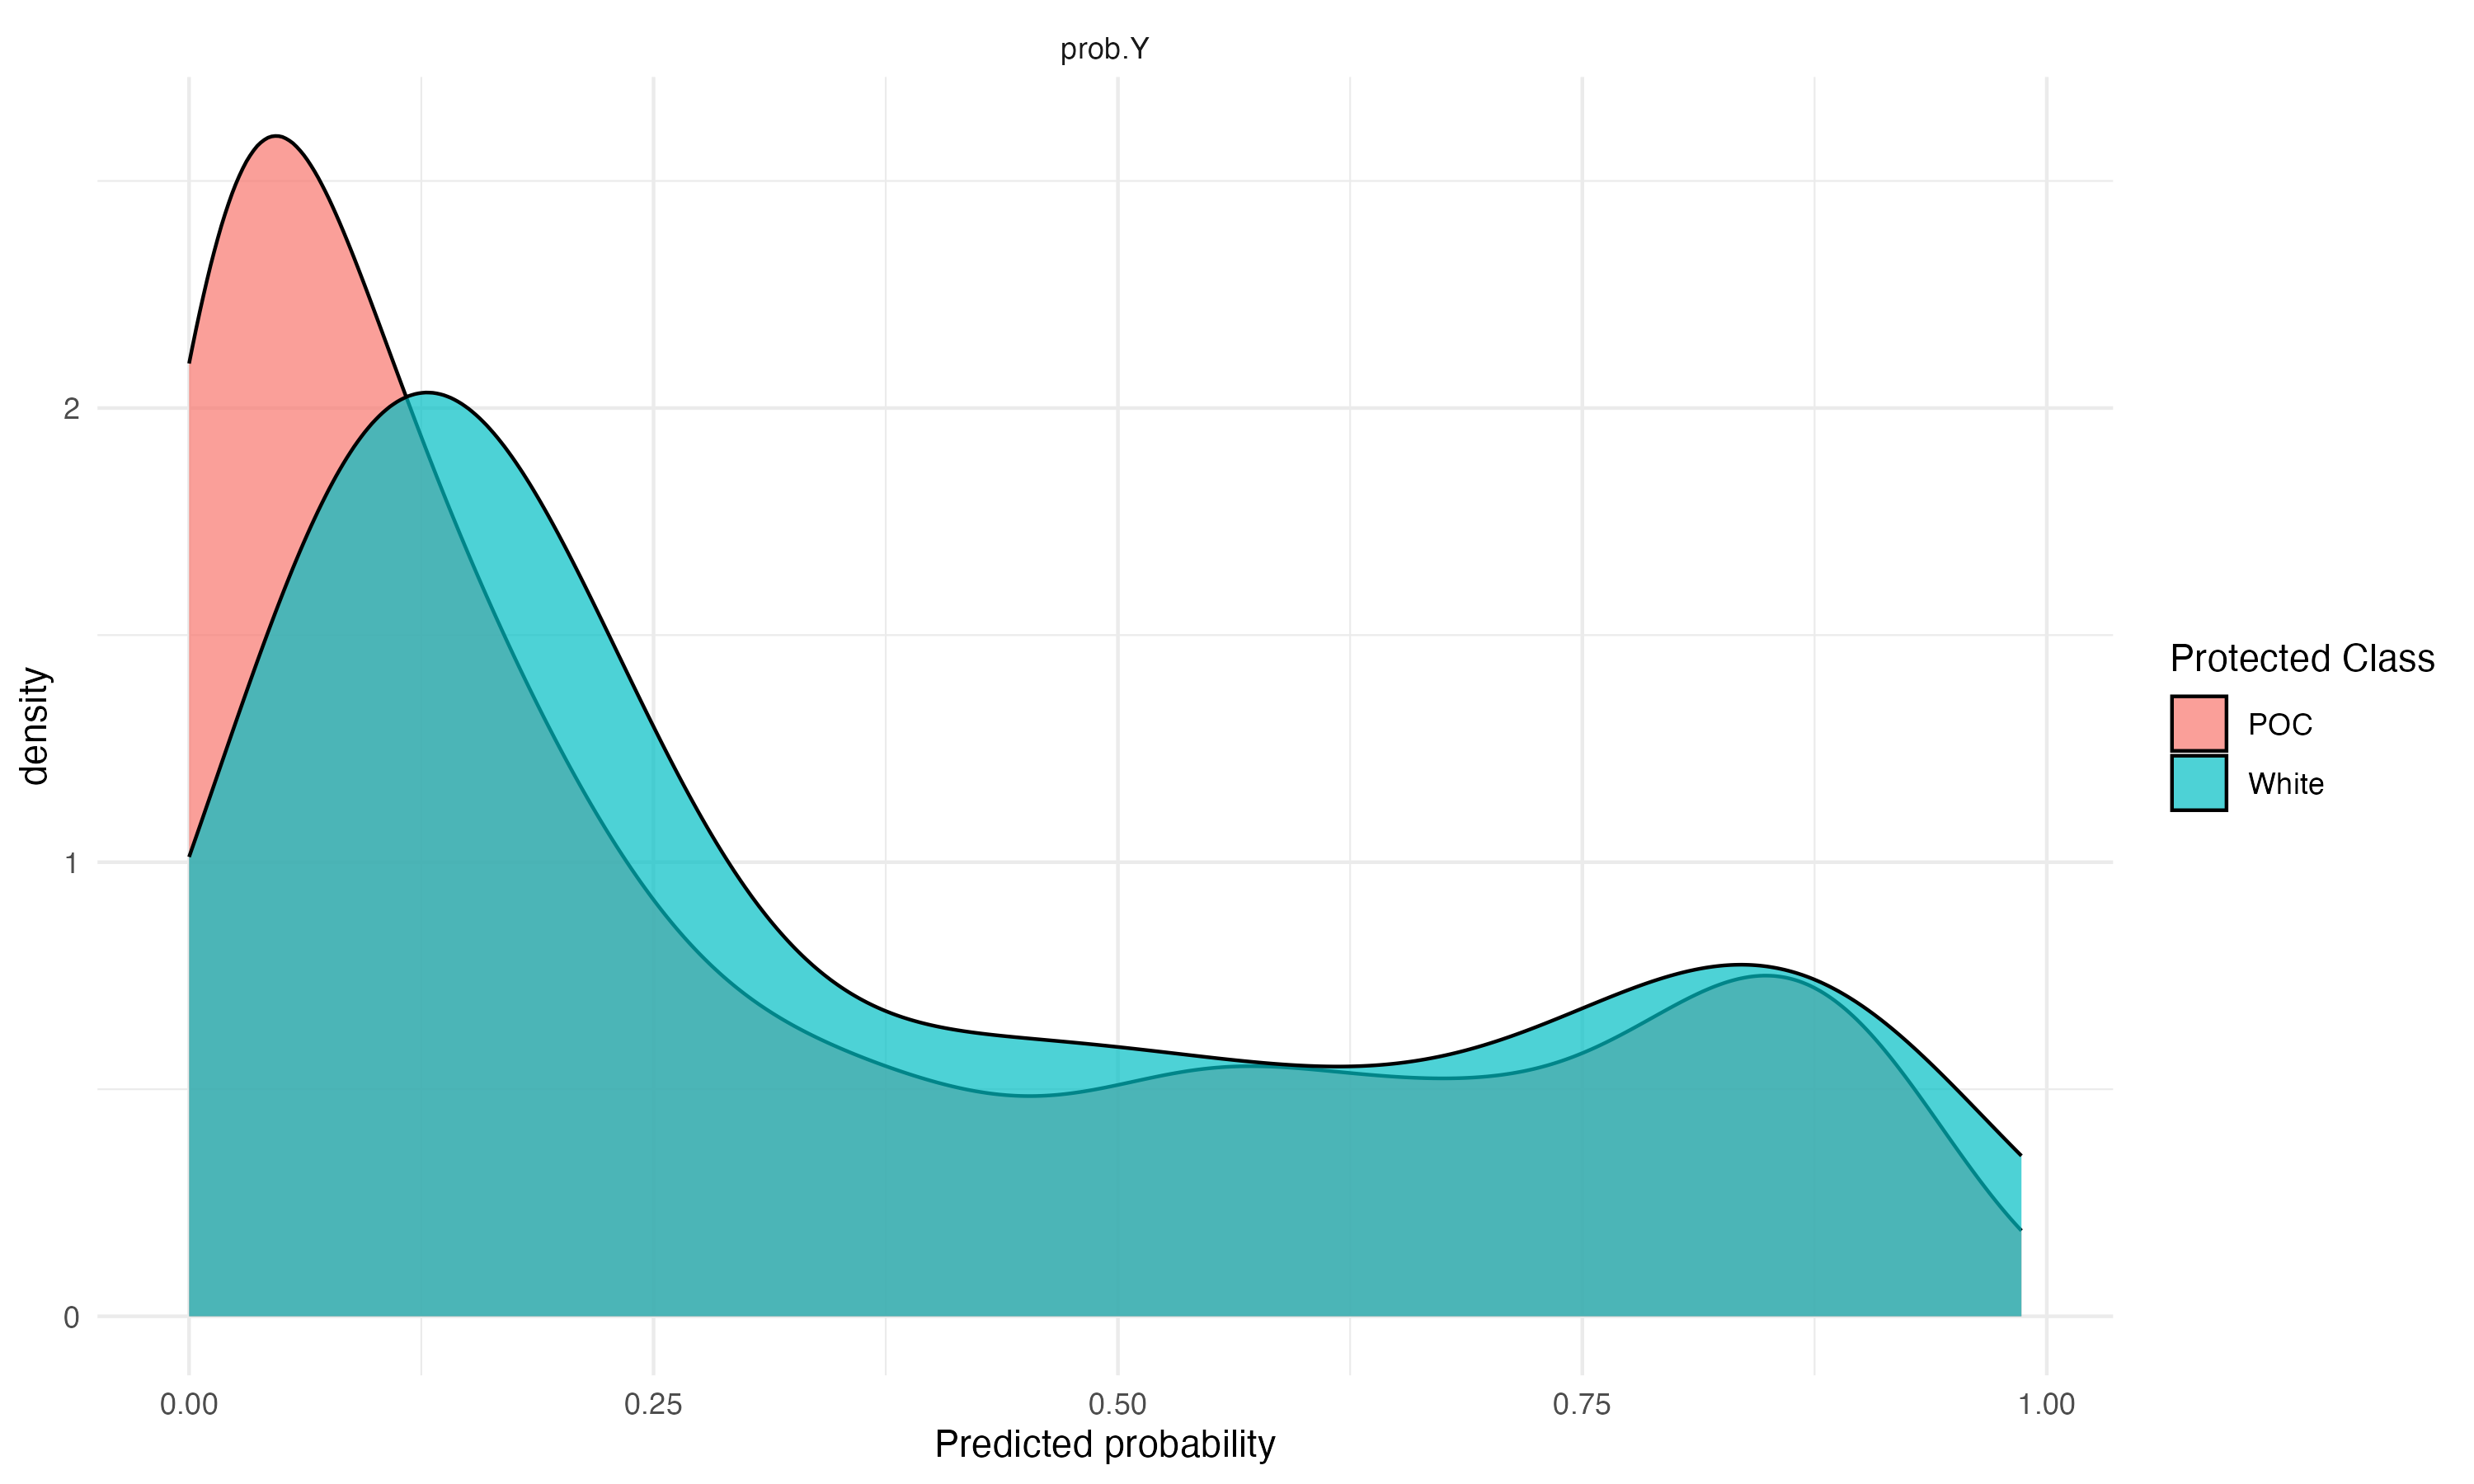
\includegraphics[width=\textwidth]{../figures/sqf_case_study_plot1.png}
        \caption{Density of predicted probabilities for both groups.}
        \label{fig:fairness_density}
    \end{minipage}
    \hfill
    \begin{minipage}{0.48\textwidth}
        \centering
        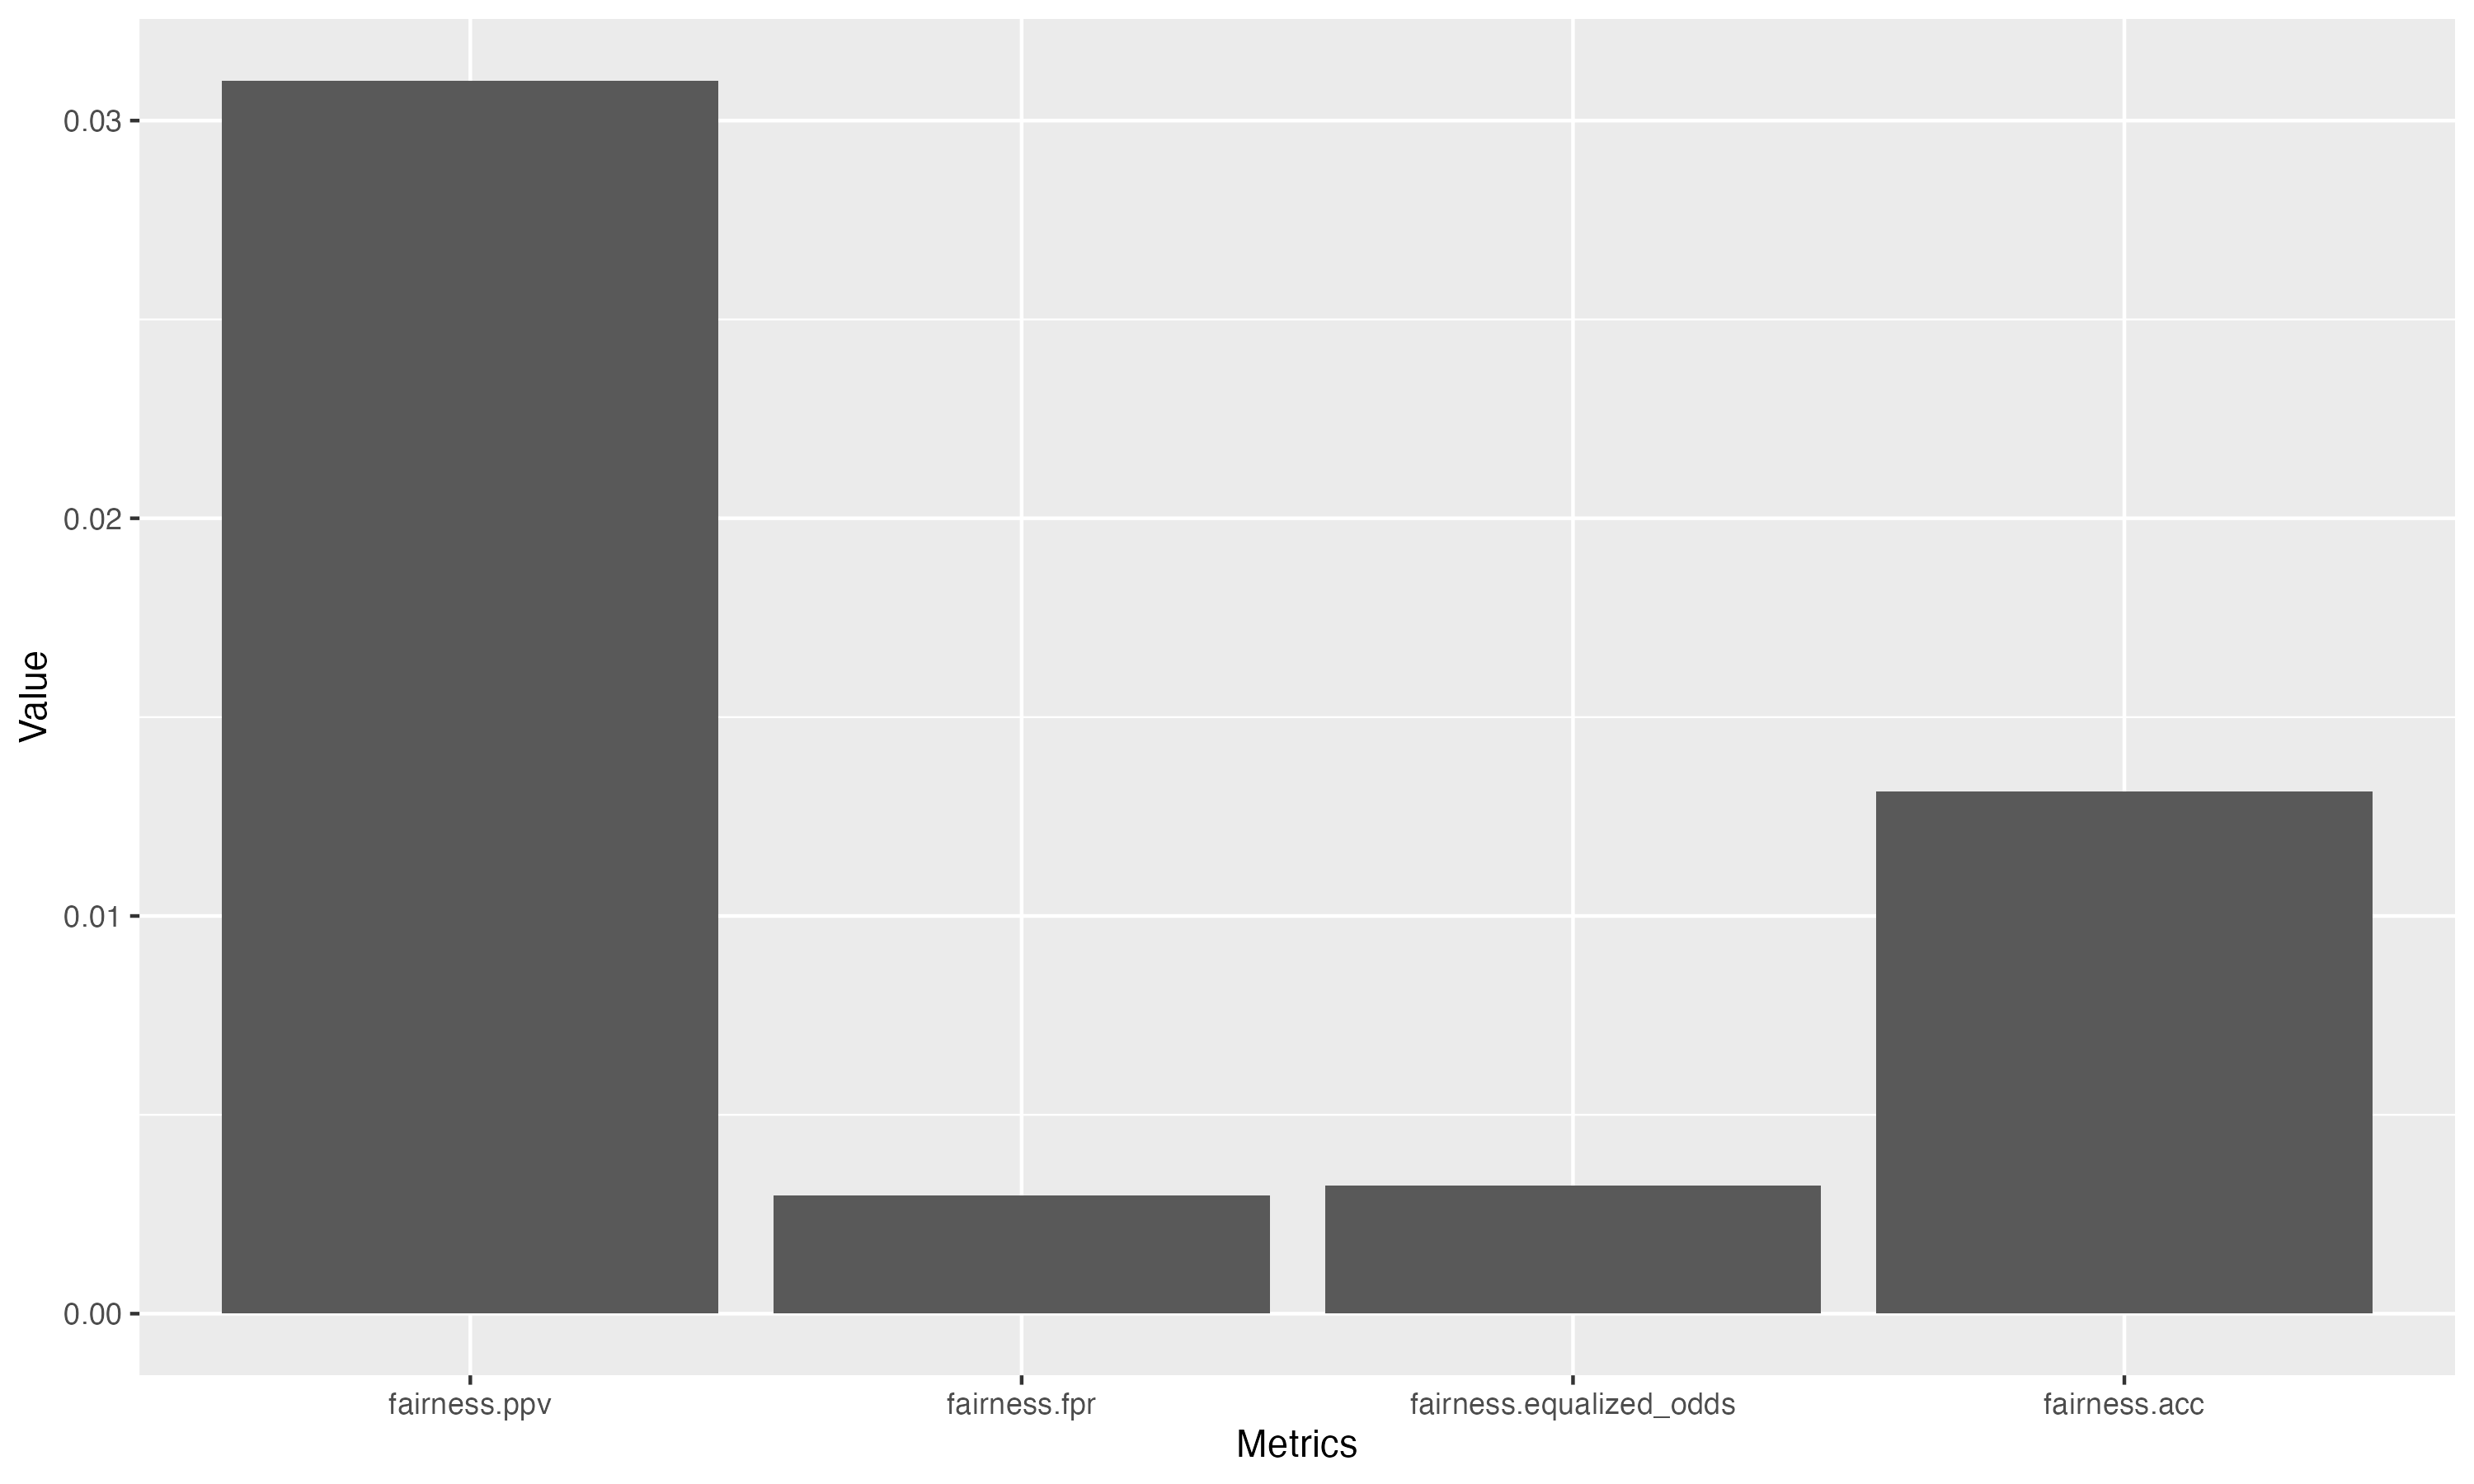
\includegraphics[width=\textwidth]{../figures/sqf_case_study_plot2.png}
        \caption{Another relevant plot.}
        \label{fig:fairness_metrics}
    \end{minipage}
\end{figure}

% results table
\begin{table}[ht]
  \centering
    \begin{tabular}{lrr}
      \hline
    Metric & PoC & White \\ 
      \hline
    tpr & 0.34 & 0.38 \\ 
      npv & 0.75 & 0.69 \\ 
      fpr & 0.07 & 0.13 \\ 
      ppv & 0.68 & 0.65 \\ 
      fdr & 0.32 & 0.35 \\ 
      acc & 0.74 & 0.68 \\ 
       \hline
    \end{tabular}
  \caption{Groupwise Fairness Metrics (2023)} 
  \label{tab:groupwise_metrics_2023}
\end{table}

\subsubsection*{Fairness Experiment}
Given that there are indeed disparities for two of the chosen metrics that exceed the $\epsilon$ threshold, we experiment with some fairness methods for the SQF data.
The \texttt{mlr3fairness} package currently has two pre-processing methods, one post-processing method and some fairness adjusted models implemented. We decide to use a reweighing methods that works with assigning weights to the observations to equalize the distribution of $P(Y|A)$.
The in-processing method is a fairness-adjusted logistic regression implemented in \texttt{mlr3fairness} inspired by Zafar et al. This method optimizes for statistical parity (Independence). The post-processing method aims for equalized odds, and it works by randomly flipping a subset of predictions with pre-computed probabilities in order to satisfy equalized odds constraints. {\color{red}{reference to mlr3fairness book}} \\
In \autoref{fig:fairness_experiment} we compare the performance and fairness of each classifier, measured by the difference in true positive rates and the classification accuracy respectively. In the bottom right corner we find fair and accurate classifiers. In terms of fairness reweighing and the equalized odds post-processing method perform best. However, the regular random forest classifier comes close to their fairness performance and performs slightly more accurate. The fairness adjusted logistic regression performs worst in terms of accuracy and fairness.
We note that this picture can of course change depending on how one measures fairness (the difference we see on the y-axis).

% result plot fairness experiment
\begin{figure}
    \centering
    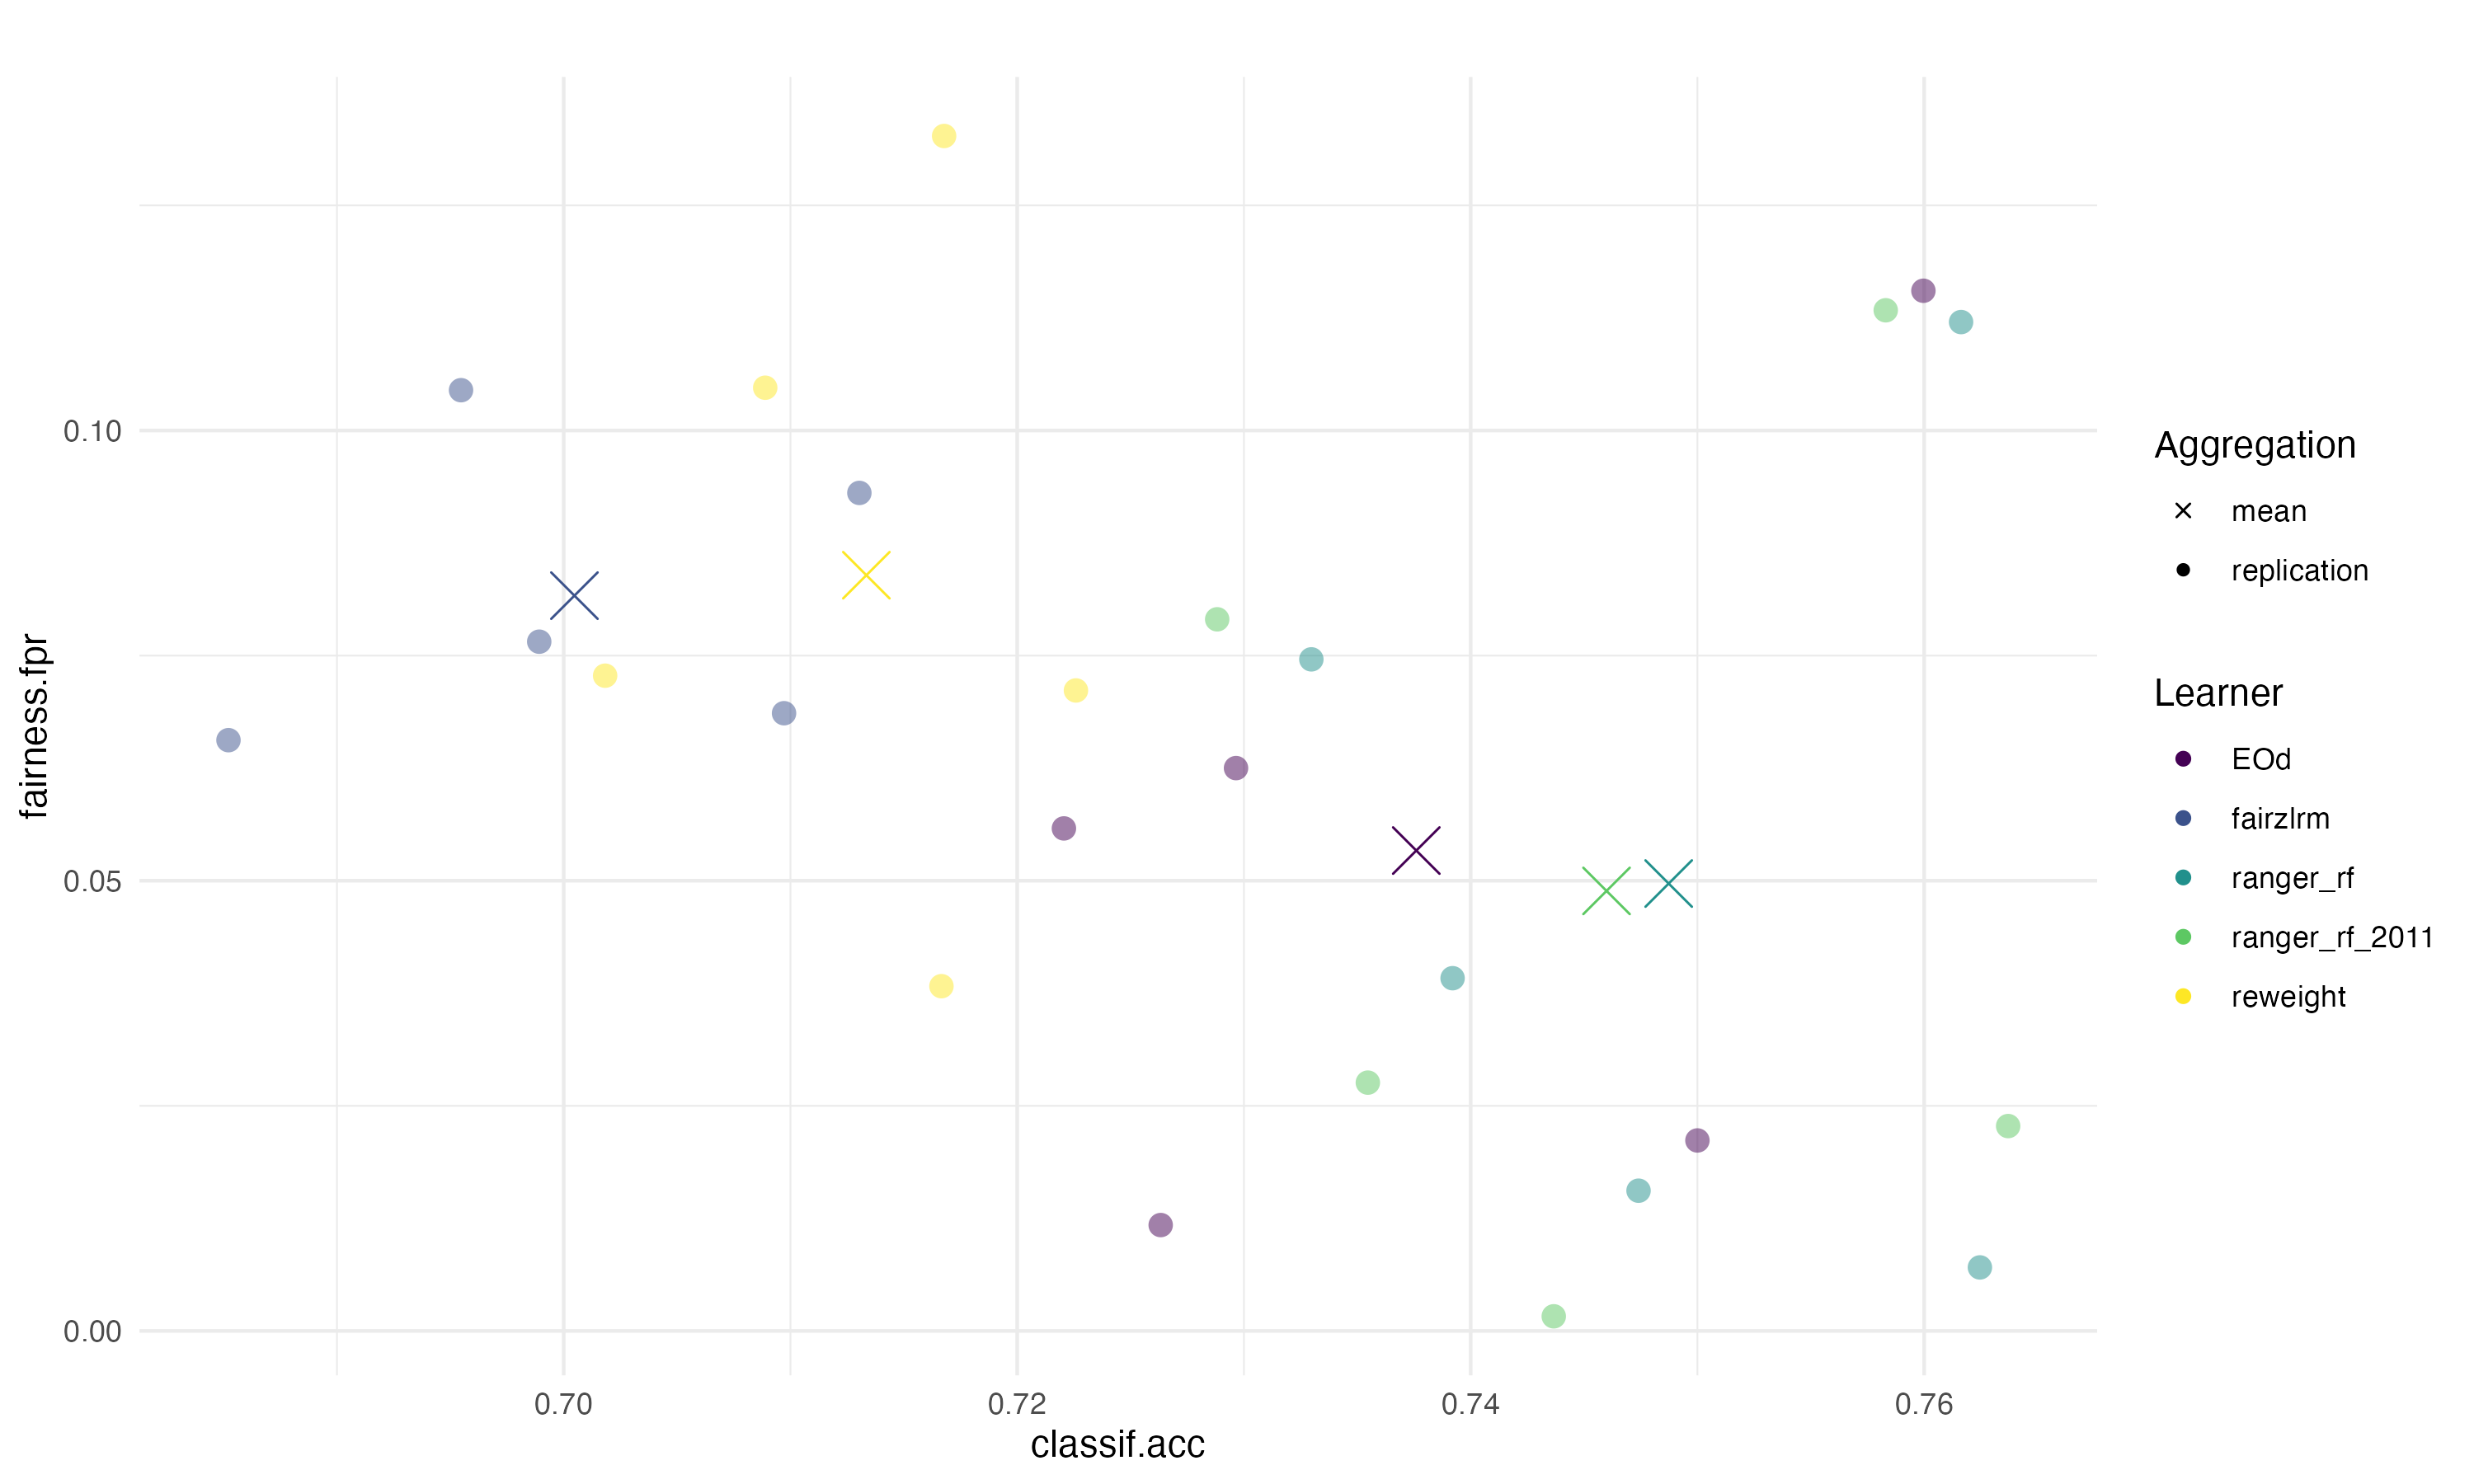
\includegraphics[width=0.7\textwidth]{../figures/sqf_case_study_plot3.png}
    \caption{Fairness metrics for the fairness adjusted random forest classifier.}
    \label{fig:fairness_experiment}
\end{figure}

\subsubsection*{Training on stops from an unconstitutional period}
Considering that the SQF practice from 2004 to 2012 has been deemed unconstitutional, the question arises whether a classifier trained on data from this period shows more racial disparities.
We choose data from 2011 as it is the year with the most stops.
We carry out the same data cleaning steps for the 2011 data as before, starting with 685724 recorded stops and reducing this to 651567 clean observations. Note that these are more than 50 times more stops than in 2023.
The 2011 data has substantially more low-risk stops, only around 6\% of stops result in an arrest. This is a stark contrast to the 2023 data, where 31\% of stops resulted in an arrest.
The differences in arrestment rate between groups are slightly lower for 2011 and the highest arrestment rate remains to be for the white group.
Due to the large proportion of low-risk stops in 2011 the predicted probabilities are generally low. In fact, the predicted probabilities for the positive class are generally so low that the classifier rarely predicts the positive class for any person, regardless of group membership.
So a classifier trained on data from the 2011 data primarily suffers from the highly skewed distribution of arrests. A reweighing technique would first need to establish more balance in the target before any fairness analysis becomes relevant.\\ 

All in all, it seems like a classifier trained on SQF data to predict the arrest of a suspect is not discriminatory against PoC. In fact, it even performs better for PoC than for white people.
To truly understand what these findings are telling us, it is crucial to take a step back and look at the context of the data and the algorithm.


% \textbf{Fairness Experiment}
% - fairness metrics (table) for dichotomised race and for full race grouping in appendix.
% - fairness methods (inspired by the article)

% Reweighing: https://mlr3fairness.mlr-org.com/reference/mlr_pipeops_reweighing.html?utm_source=chatgpt.com#format
% Fair logistic regression: https://rdrr.io/cran/mlr3fairness/man/mlr_learners_classif.fairzlrm.html?utm_source=chatgpt.com
% EOd: https://mlr3fairness.mlr-org.com/reference/mlr_pipeops_equalized_odds.html?utm_source=chatgpt.com
% mlr3book: https://mlr3book.mlr-org.com/chapters/chapter14/algorithmic_fairness.html?utm_source=chatgpt.com#bias-and-fairness
% https://mlr3fairness.mlr-org.com/#debiasing-methods



% The data introduced three main challenges: selection bias; missing data; class imbalance.



% borough specific graphics?

% - number of stops conducted but with background information who governed at that time (see Obsidian)
% - transparent explanation of feature selection (similar to Data Transparanecy paper)
% - distribution of race in SQF data vs NYC
% - grouping to black, white, black hispanic, white hispanic, others --> arrestment rates in these groups


